\clearpage
\chapter{Mastery Workbook 1}

% Chapter page
\section{Logic And Reasoning Mastery Workbook}

\horizontalline{0}{0}

\begin{center}
    \Large{\textbf{I have neither given nor received unauthorized assistance.}}
    \horizontalline{0}{0}
    \large{\textbf{Taylor James Larrechea}}
    \horizontalline{0}{0}
\end{center}

% Problem 1
\begin{problem}{Problem 1}
    \begin{statement}{Problem Statement}
        \begin{itemize}
            \item Solve the following.
            \item Describe, as carefully as you can, your process for solving.
            \item Are you using inductive or deductive reasoning?
            \item Can you be sure your answer is correct?
        \end{itemize}

        \begin{center}
            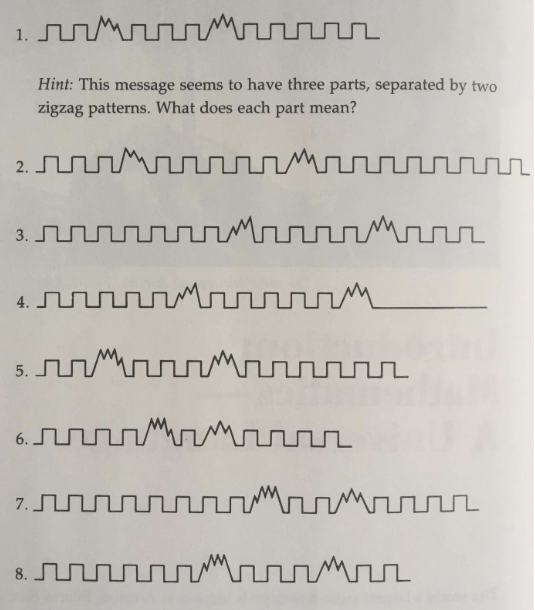
\includegraphics[width=0.5\textwidth]{./Images/Math Signals.png}
        \end{center}

    \end{statement}

    In this problem, the diagrams that are being depicted depict arithmetic in mathematics. The square waves represent integer values and the little mountain looking symbols represent a mathematical
    operation. To begin, we look at the first two diagrams.


    \begin{Highlight}{Diagram 1 \& 2}
        These diagrams are depicting addition. In english terms we have two plus three equals five. The first mountain represents plus and the second mountain represents the equals symbol.

        \setcounter{equation}{0}
        \begin{equation}
            2 + 3 = 5
        \end{equation}
        \qed

        Now, we look at the next diagram, diagram 2.
        \begin{equation}
            3 + 5 = 8
        \end{equation}
        \qed
    \end{Highlight}

    We now look at the next two diagrams, diagram 3 and 4.

    \begin{Highlight}{Diagram 3 \& 4}
        These diagrams are depicting subtraction. Here, the first mountain is reversed to that of the first two diagrams. Since subtraction is the opposite of addition, we have the following statements.

        \begin{equation}
            7 - 4 = 3
        \end{equation}
        \qed

        Now, we look at the next diagram, diagram 4.

        \begin{equation}
            5 - 5 = 0
        \end{equation}
        \qed
    \end{Highlight}

    We now look at the next two diagrams, diagram 5 and 6.

    \begin{Highlight}{Diagram 5 \& 6}
        These diagrams are depicting multiplication. The first mountain peak is now indicative of a multiplication symbol. With this new logic we can make the following statements.

        \begin{equation}
            2 \times 3 = 6
        \end{equation}
        \qed

        Now, we look at the next diagram, diagram 6.

        \begin{equation}
            4 \times 1 = 4
        \end{equation}
        \qed
    \end{Highlight}

    Lastly, we exam the final two diagrams, 7 and 8.

    \begin{Highlight}{Diagrams 7 \& 8}
        Similar to that of the first four diagrams, diagram 7 and 8 are related to that of 5 and 6 in that the operations of 7 and 8 are the inverse of 5 and 6. This means that the first
        mountain valley is indicative of division. With this in mind, we can make the following statements for the last two diagrams.

        \begin{equation}
            8 / 2 = 4
        \end{equation}
        \qed

        \begin{equation}
            6 / 3 = 2
        \end{equation}
        \qed
    \end{Highlight}
\end{problem}

% Problem 1 Summary

\begin{summary}{Problem 1 Summary}
    \begin{statement}{Procedure}
        \begin{itemize}
            \item Count the number of `square waves' and `peaks' in each line
            \item Make an educated guess what each symbol means in the given diagram
            \item Infer what the given operation of symbols mean, and test this inference on other diagrams
        \end{itemize}
    \end{statement}
    \begin{statement}{Key Concepts}
        \begin{itemize}
            \item This problem utilizes \textbf{inductive reasoning} by recognizing patterns and making hypothesis' about what the symbols in diagrams represent
            \item After a hypothesis has been checked and confirmed, we use \textbf{deductive reasoning} to determine what other diagrams represent
        \end{itemize}
    \end{statement}
    \begin{statement}{Variations}
        \begin{itemize}
            \item We could be given the same symbols with different values that each diagram is to represent
            \begin{itemize}
                \item In this case we would use our established definitions for symbols and determine what the result is from the new diagram
            \end{itemize}
            \item We could be given a different set of diagrams with new symbols
            \begin{itemize}
                \item In this case we would use the same procedure from our previous set of diagrams to determine what the values are from the patterns
            \end{itemize}
        \end{itemize}
    \end{statement}
\end{summary}

% Problem 2
\begin{problem}{Problem 2}
    \begin{statement}{Problem Statement}
        Translate the tablets below. Describe your process of solving in detail. Are you using inductive or deductive reasoning? Can you be sure your answer is correct?

        \begin{center}
            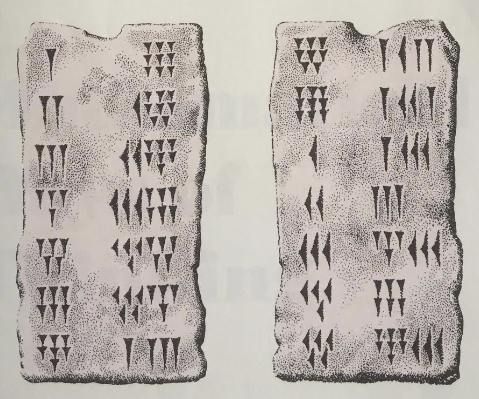
\includegraphics[width = 0.5\textwidth]{"./Images/Babylonian Tablet.png"}
        \end{center}
    \end{statement}

    \begin{Highlight}[Solution]
        The tablet depicted above is an example of a early multiplication table found in Babylonian times. This table is taking the values on the left hand column and multiplying them by nine. This 
        particular table can be translated from left to right top to bottom:

        \begin{eqnarray*}
            1 \times 9 = 9 \\
            2 \times 9 = 18 \\
            3 \times 9 = 27 \\
            4 \times 9 = 36 \\
            5 \times 9 = 45 \\
            6 \times 9 = 54 \\
            7 \times 9 = 63 \\
            8 \times 9 = 72 \\
            9 \times 9 = 81 \\
            10 \times 9 = 90 \\
            20 \times 9 = 180 \\
            30 \times 9 = 270 \\
            40 \times 9 = 360 \\
            50 \times 9 = 450 \\
        \end{eqnarray*}

        The number system that is being used on these tablets is base 60. The `golf tee' looking symbols are equal to different values depending on the number that is being represented. The `left arrow'
        key looking symbols represent 10. Take for instance the third line of the tablet on the left. Here we see the first column having three units representing the number three and the second column
        having two arrow key symbols (adding up to 20) and seven golf tee symbols adding up to 7. In the manner that these are placed, the number on the second column represents 27.

        Now, when we get to the second tablet, when the value of the multiplication exceeds 60, the golf tees that come before the left arrow keys represent units of 60. The arrow key still represents 10
        but the golf keys that succeed the arrow key are counted as units of 1. Take for instance the second line of the second tablet. On the first column we have nine golf tees representing nine. On the
        second column we have a golf tee representing 60, two arrow keys both representing 10, and another golf tee that succeeds the arrow keys representing one. This in turn reads as $9 \times 9 = 81$ where
        81 is found by adding up the value of each symbol from left to right of the second column.

        I found this pattern by observing the differences between lines and drawing a connection between the values on the left hand and right hand sides of the first tablet. After this was, when I got above
        the value of 60, I had to draw connections between what the symbols now represented. I went with my initial inclination that this was a multiplication table by nine and then filled in the gaps for
        what these symbols are being reconstructed to mean. It was only after I got above the value of 60 that I was able to determine that the symbols had a different value depending on where they were written
        in the line.

        I used deductive reasoning to figure out what each symbol meant from line to line of the tablet. After getting a grasp of the values that were below 60, I had to reformulate what I was thinking the values
        were and then draw connections between an assumption and then what they actually were equivalent to. Early on in the process I was using more deductive reasoning, but once I found a pattern I used deductive
        reasoning to draw final conclusions.
    \end{Highlight}
\end{problem}

% Problem 2 Summary
\begin{summary}{Problem 2 Summary}
    \begin{statement}{Procedure}
        \begin{itemize}
            \item This problem uses the same procedure that was used to solve problem 1 of this assignment
            \item First, make a hypothesis for what a symbol represents and then test that hypothesis on a different set of symbols
            \item Repeatedly test this hypothesis until it is confirmed to be true or false and then change if needed
        \end{itemize}
    \end{statement}
    \begin{statement}{Key Concepts}
        \begin{itemize}
            \item This problem utilizes \textbf{inductive reasoning} to make inferences as to what a pattern of symbols means
            \item After the hypothesis has been checked and confirmed, we can use \textbf{deductive reasoning} to then determine what other patterns represent with the same symbols
        \end{itemize}
    \end{statement}
    \begin{statement}{Variations}
        \begin{itemize}
            \item Similar to problem 1, we could be given a pattern with the same definition of symbols as depicted in this problem
            \begin{itemize}
                \item In this case we would use the definition of symbols to determine what the new pattern equates to in terms of numerical value
            \end{itemize}
            \item We could be given a new set of symbols that represent different definitions in different patterns
            \begin{itemize}
                \item In this case we would use the same procedure from this problem to determine what these new symbols represent and make a hypothesis on what they mean, test the hypothesis, and 
                come to a conclusion as to what they represent
            \end{itemize}
        \end{itemize}
    \end{statement}
\end{summary}

% Problem 3
\begin{problem}{Problem 3}
    \begin{statement}{Problem Statement}
        Imagine you are given 3 matchboxes, labeled “Red and White,” “Red and Red,” and “White and White.” Each box contains 2 marbles which can be either red or white. The labels on each box are 
        incorrect  (although the labels would be correct if you switched them around). You are allowed to peek inside one box and look at exactly one marble in that box - and see if it is red or white.

        \begin{itemize}
            \item After this, can you figure out what is in each box and fix the labels to be correct?
            \item Does it matter which box you choose to open at the start?
            \item Are you using inductive or deductive reasoning?
            \item Can you be sure of your answer?
        \end{itemize}
    \end{statement}
    
    \begin{Highlight}[Solution]
        I am first going to make some assumptions. The player in this game knows that the boxes are incorrectly labeled and after they look at the first marble in the box, they can switch the labels on
        the box as many times as their heart desires. With these assumptions, I will now answer the following questions. \vspace*{1em}

        \noindent \textbf{After this, can you figure out what is in each box and fix the labels to be correct?} \vspace*{1em}

        After the player opens the box that is incorrectly labeled (this is important that the player knows that they are incorrectly labeled) they are allowed to look at one marble. The player then makes
        an assumption of what the other marbles color is and will switch labels on the box according to their assumption.

        If the player correctly assumes the other color of the marble, then they will switch the current label on the box with that of their assumed correct label of the box. The player at this point believes
        that they have correctly labeled the first box. They still know intrinsically that the other box that has not had its labeled switched is still incorrect. This then means that the player has to switch 
        that boxes label with that of the other box that originally switched with and in turn they correctly label each box.

        Now, if the player incorrectly identifies the other marbles color they will now incorrectly label their current box again when they switch labels with their incorrectly assumed label of the current box.
        Deep down they know that they still have one box that is incorrectly labeled, so they switch the remaining two boxes labels again. This causes a problem because the player has once again incorrectly labeled
        every box on the table.

        The only way a player will correctly label each box is if they correctly assume the color of the other marble and then only make two switches of the labels. If they incorrectly switch the label of the
        current box because they incorrectly assumed the color of the other marble, then they will have three boxes that are incorrectly labeled.

        There is not definitive way that a player can know if they have correctly labeled each box. It is possible that a player can correctly label each box, but that is contingent upon them correctly identifying
        the other marble in the box and knowing that each box was incorrectly labeled from the beginning. This is of course assuming that the player is opening up any of the boxes.

        \begin{center}
            \textbf{They can, but only if they correctly identify the other marble in the box.}
        \end{center}

        \noindent \textbf{Does it matter which box you choose to open at the start?} \vspace*{1em}

        If the player goes into the game knowing that the boxes are all incorrectly labeled, the box that they should examine is that of the box that is labeled as \textbf{red / white}. This is because when the player
        opens this box, they will either see a white or red marble because in order for this label to be incorrectly labeled it has to be on the red / red box or the white / white box. If they open up this box and see
        a marble, they can automatically assume that the other marble is of the same color based on the prior knowledge that the boxes were all incorrectly labeled. The player then switches the label of the current box
        with that of either the white / white or red / red label and then switches the other remaining box with that of the box that they just switched labels with. 

        \begin{center}
            \textbf{The player should open the box that is incorrectly labeled with the red / white label.}
        \end{center}

        \noindent \textbf{Are you using inductive or deductive reasoning?} \vspace*{1em}

        If the player is following the advice of opening the box with the red / white label, then they are using deductive reasoning because they know by default that all the boxes are incorrectly labeled. By opening this
        box they know immediately what the other marbles color is and they can first switch labels so that this box is correctly labeled. Then, if they also know that the other box was incorrectly labeled from the start, they
        can switch labels again to assure that every box now has their correct labels.

        \begin{center}
            \textbf{This is using deductive reasoning.}
        \end{center}

        \noindent \textbf{Can you be sure of your answer?} \vspace*{1em}

        As previously mentioned, if the player opens the box that is labeled as red / white, they can be sure that each box is correctly labeled after two permutations of label switching. If they do not follow this strategy,
        they cannot explicitly know if they are correct.

    \end{Highlight}
\end{problem}

% Problem 3 Summary
\begin{summary}{Problem 3 Summary}
    \begin{statement}{Procedure}
        \begin{itemize}
            \item First determine what it means to open a box that is labeled as `red / white'
            \item Figure out what it means to switch labels and what boxes will remain incorrectly labeled
            \item Figure out how a player can correctly label the other two boxes without knowing what is inside those boxes
        \end{itemize}
    \end{statement}
    \begin{statement}{Key Concepts}
        \begin{itemize}
            \item This problem uses \textbf{deductive reasoning} from a set of rules as to how the game is played
            \item A strategy is developed for solving this puzzle based on the what box a player should open first and what marble they observe
            \item Because we know that every box is incorrectly labeled, we can then determine what labels need to be switched based off of the first box that is opened by the player
        \end{itemize}
    \end{statement}
    \begin{statement}{Variations}
        \begin{itemize}
            \item We can be given a different riddle with a set of concrete rules as to how the game is played
            \begin{itemize}
                \item We would then have to make a hypothesis and test that hypothesis based off the rule of the game, and then test it to see if we got the desired result
                \item All possibilities must be tested to make a final determination of what the correct answer to the problem would be
            \end{itemize}
        \end{itemize}
    \end{statement}
\end{summary}

% Problem 4
\begin{problem}{Problem 4}
    \begin{statement}{Problem Statement}
        At a famous pizza place, Albert, Bob, and Jose are asked by a waiter, “Does everybody want water?” Albert says “I don’t know.”  Bob then says, “I don’t know.” Jose says, “Not everyone wants water.” 
        The waiter returns and brings correctly each person what they wanted.  Which people got water?

        Be sure to explain how you reached your conclusion. HINTS: Pay close attention to the specific question the waiter asks.  Assume everyone involved has a firm grasp on propositional logic. And that no 
        one knows what the others want before they speak. Also, you do not need to use truth tables, but you must use a clear deductive argument.
    \end{statement}

    \begin{Highlight}[Solution]
        The waiter specifically asked \underline{`Does everyone want water?'}. By asking this question, the waiter is specifically is trying to determine whether or not Albert, Bob, and Jose all want water.
        Let's now examine what each person said at the table and what it implies.

        \begin{itemize}
            \item \textbf{Albert} - Albert responds with \underline{`I don't know'}. This implies that Albert doesn't necessarily know if everyone at the table wants water.
            \item \textbf{Bob} - Bob responds with the same answer as Albert. The same logic for what he wants to drink applies to himself as it did to Albert.
            \item \textbf{Jose} - Jose responds with \underline{`Not everyone wants water'}. This implies that there are people at the table that what want water, but not all of them.
        \end{itemize}

        Let's break this down a little further. Albert initially says he doesn't know if everyone wants water. If he himself wants water, he doesn't know if Bob and Jose want water as well. If he doesn't
        want water, he then would know that not everyone wants water. Because of this, we know that \textbf{Albert does want water}.

        Bob says the same thing as Albert implying that if he doesn't want water, he would know that not everyone wants water and that too would contradict what he said to the waiter. This means that he too could
        want water, but he doesn't know if the other two want water as well. \textbf{Bob does not want water}.

        Jose's response indicates that he knows that not everyone at the table wants water. Because of the way that Albert and Bob answered, if they answered that they didn't want water, they would actually know
        that not everyone at the table wants water. Since they did not know if everyone wanted water in combination with Jose's response, the only logical person to receive water would be Jose. \textbf{Jose wants
        water}.

        \begin{center}
            \textbf{Albert and Jose want water, Bob does not.}
        \end{center}
    \end{Highlight}
\end{problem}

% Problem 4 Summary
\begin{summary}{Problem 4 Summary}
    \begin{statement}{Procedure}
        \begin{itemize}
            \item First examine what the phrase `Does everybody want water?' means
            \item Carefully examine what each person responds with and what that implies with the original statement
            \item Use logical reasoning to deduce what each person wants with respect to how they respond to the prompt
        \end{itemize}
    \end{statement}
    \begin{statement}{Key Concepts}
        \begin{itemize}
            \item This problem utilizes \textbf{deductive reasoning} by observing each persons response to the original prompt
            \item We then make logical connections as to what each persons response means in regards to the original phrase by the waiter
        \end{itemize}
    \end{statement}
    \begin{statement}{Variations}
        \begin{itemize}
            \item The original phrase could be changed from the waiter
            \begin{itemize}
                \item We would then have to use the same logic in examining each persons response as to what it means in regards to the phrase from the waiter
            \end{itemize}
            \item The responses from the patrons could be changed
            \begin{itemize}
                \item We would then have to use the same logic in examining each persons response to the waiters original phrase
            \end{itemize}
            \item A completely different set of questions and responses could be presented to this group
            \begin{itemize}
                \item Again, we would then have to use the same logic of examining each persons response to determine what it is that they want
            \end{itemize}
        \end{itemize}
    \end{statement}
\end{summary}

% Problem 5
\begin{problem}{Problem 5}
    \begin{statement}{Problem Statement}
        Let p and q be the propositions:

        \begin{itemize}
            \item p : I bought a lottery ticket this week.
            \item q : I won the million dollar jackpot.
        \end{itemize}

        Express each of these propositions as an English sentence.

        \begin{enumerate}[label=(\alph*)]
            \item $\neg p$
            \item $p \vee q$
            \item $p \rightarrow q$
            \item $p \wedge q$
            \item $p \leftrightarrow q$
            \item $\neg p \rightarrow \neg q$
            \item $\neg p \wedge \neg q$
            \item $\neg p \vee (p \wedge q)$
        \end{enumerate}
    \end{statement}

    \begin{Highlight}[Solution - Parts (a) - (h)]
        The solutions for the following parts can be seen below.
        \begin{enumerate}[label=(\alph*)]
            \item $\mathbf{\neg p}$ - I did not buy a lottery ticket this week.
            \item $\mathbf{(p \vee q)}$ - I bought a lottery ticket this week or I won the million dollar jackpot.
            \item $\mathbf{(p \rightarrow q)}$ - If I buy a lottery ticket this week, then I will win the million dollar jackpot.
            \item $\mathbf{(p \wedge q)}$ - I bought a lottery ticket this week and I won the million dollar jackpot.
            \item $\mathbf{(p \leftrightarrow q)}$ - I bought a lottery ticket if and only if I won the million dollar jackpot.
            \item $\mathbf{(\neg p \rightarrow \neg q)}$ - If I did not buy a lottery ticket this week, then I have not won the million dollar jackpot.
            \item $\mathbf{(\neg p \wedge \neg q)}$ - I did not buy a lottery ticket this week and I did not win the million dollar jackpot.
            \item $\mathbf{(\neg p \vee (p \wedge q))}$ - I did not buy a lottery ticket this week or I bought a lottery ticket this week and I won the million dollar jackpot.
        \end{enumerate}
    \end{Highlight}
\end{problem}

% Problem 5
\begin{summary}{Problem 5 Summary}
    \begin{statement}{Procedure}
        \begin{itemize}
            \item When presented with a negation ($\neg$), we simply find the inverse of a given proposition
            \item When presented with a disjunction ($\vee$), we simply connect two propositions with the word `or'
            \item When presented with a conjunction ($\wedge$), we simply connect two propositions with the word `and'
            \item When presented with a conditional ($\rightarrow$), we simply connect two propositions with the terms `if' and `then'
            \item When presented with a bi-conditional ($\leftrightarrow$), we simply connect two propositions with the term `if and only if'
        \end{itemize}
    \end{statement}
    \begin{statement}{Key Concepts}
        \begin{itemize}
            \item This problem utilizes logical connectives to from sentences in English from two propositions
            \item This problem takes into account how to use logical connectives in the context of forming English statements
        \end{itemize}
    \end{statement}
    \begin{statement}{Variations}
        \begin{itemize}
            \item The propositions that are given to us could be changed
            \begin{itemize}
                \item In this case we would use the same procedure in forming English statements based off of the logical connectives that are presented to us
            \end{itemize}
            \item We could be given different propositional logic statements with the same propositions
            \begin{itemize}
                \item In this case we would still use the procedure for representing propositions with logical connectives 
            \end{itemize}
            \item We could be given different propositional logic statements with different propositions
            \begin{itemize}
                \item In this case we would still use the same procedure for connecting propositions with logical connectives in English statements
            \end{itemize}
        \end{itemize}
    \end{statement}
\end{summary}

% Problem 6
\begin{problem}{Problem 6}
    \begin{statement}{Problem Statement}
        Construct a truth table for each of these compound propositions. \textbf{Only submit d.}

        \begin{enumerate}[label=(\alph*)]
            \item $p \wedge \neg p$
            \item $p \vee \neg p$
            \item $(p \vee \neg q) \rightarrow q$
            \item $(p \vee q) \rightarrow (p \wedge q)$
            \item $(p \rightarrow q) \leftrightarrow (\neg q \rightarrow \neg p)$
            \item $(p \rightarrow q) \rightarrow (q \rightarrow p)$
        \end{enumerate}
    \end{statement}

    \begin{Highlight}[Solution - Part (d)]
        The truth table for part (d) of this problem can be seen below.

        \begin{center}
            \begin{tabular}[h]{|c|c|c|c|c|}
                \hline $\mathbf{p}$ & $\mathbf{q}$ & $\mathbf{(p \vee q)}$ & $\mathbf{(p \wedge q)}$ & $\mathbf{(p \vee q)} \rightarrow \mathbf{(p \wedge q)}$ \\ \hline
                T & T & T & T & T \\ \hline
                T & F & T & F & F \\ \hline
                F & T & T & F & F \\ \hline
                F & F & F & F & T \\ \hline
            \end{tabular}
        \end{center}
    \end{Highlight}
\end{problem}

% Problem 6 Summary
\begin{summary}{Problem 6 Summary}
    \begin{statement}{Procedure}
        \begin{itemize}
            \item Use the definition of truth values with propositions with logical connectives such as ($\wedge$), ($\vee$), and ($\rightarrow$)
        \end{itemize}
    \end{statement}
    \begin{statement}{Key Concepts}
        \begin{itemize}
            \item This problem utilizes the truth value of logical connectives with propositions
        \end{itemize}
    \end{statement}
    \begin{statement}{Variations}
        \begin{itemize}
            \item We could be given a different truth table with different logical connectives
            \begin{itemize}
                \item We then use the same truth value for a logical connective for a given set of propositions
            \end{itemize}
        \end{itemize}
    \end{statement}
\end{summary}

% Problem 7
\begin{problem}{Problem 7}
    \begin{statement}{Problem Statement}
        Write the definitions of converse, contrapositive, and the inverse in a format that is useful for you to reference - make a poster, index cards, or even make notes in your book.
    \end{statement}
    
    \begin{Highlight}[Solution]
        My definitions to the above in the problem statement  can be seen below.

        \begin{itemize}
            \item \textbf{Converse} - A converse statement is a statement that switches the order of propositions in a statement. So if the original statement is `If P then Q', then 
            the converse is `If Q then P'.
            \item \textbf{Contrapositive} - A contrapositive statement is a statement that switches the order of propositions in a statement and takes the negation of each statement. This
            means that if the original statement is `If P then Q', the contrapositive statement would be `If not Q then not P'.
            \item \textbf{Inverse} - An inverse statement is a statement that takes the negation of the propositions in a statement. This means that if the original statement is `If P then Q',
            the inverse statement would be `If not P then not Q'.
        \end{itemize}
    \end{Highlight}
\end{problem}

% Problem 7 Summary
\begin{summary}{Problem 7 Summary}
    \begin{statement}{Procedure}
        \begin{itemize}
            \item Use the definition of \textbf{converse}, \textbf{contrapositive}, and \textbf{inverse} to formulate a custom definition of what each one means in the context of a logical statement
        \end{itemize}
    \end{statement}
    \begin{statement}{Key Concepts}
        \begin{itemize}
            \item This problem utilizes making a custom definition of terms that have a concrete definition, such as \textbf{converse}, \textbf{contrapositive}, and \textbf{inverse}
            \item \textbf{Converse} statements switch the order of propositions and do not have the same truth value as the original statement
            \item \textbf{Constrapositive} statements negate each proposition and switch the order of them and have the same truth value as the original statement
            \item \textbf{Inverse} statements negate each proposition and do not have the same truth value as the original statement
        \end{itemize}
    \end{statement}
    \begin{statement}{Variations}
        \begin{itemize}
            \item We could be asked to make definitions for other terms
            \begin{itemize}
                \item We would then use the same procedure in making custom definitions for said term with a concrete definition
            \end{itemize}
        \end{itemize}
    \end{statement}
\end{summary}

% Problem 8
\begin{problem}{Problem 8}
    \begin{statement}{Problem Statement}
        Write up your own conditional example, like `If it is raining, the grass is wet.' but more interesting and memorable. Write the converse, contrapositive, and the inverse of your example.
    \end{statement}

    \begin{Highlight}[Solution]
        For my conditional example, I have decided to include one of my favorite movies, Shrek. The conditional statement is as follows:

        \begin{center}
            \textbf{If you know the muffin man, then you know who Shrek is.}
        \end{center}

        \subsubsection*{Converse Statement}

        \begin{itemize}
            \item Original Statement: If you know the muffin man, you know who Shrek is.
            \item \textbf{Converse Statement: If you know who Shrek is, then you know the muffin man.}
        \end{itemize}

        \subsubsection*{Contrapositive Statement}

        \begin{itemize}
            \item Original Statement: If you know the muffin man, you know who Shrek is.
            \item \textbf{Converse Statement: If you don't know who Shrek is, then you don't know the muffin man.}
        \end{itemize}

        \subsubsection*{Inverse Statement}

        \begin{itemize}
            \item Original Statement: If you know the muffin man, you know who Shrek is.
            \item \textbf{Inverse Statement: If you don't know the muffin man, then you don't know who Shrek is.}
        \end{itemize}
    \end{Highlight}
\end{problem}

% Problem 8 Summary
\begin{summary}{Problem 8 Summary}
    \begin{statement}{Procedure}
        \begin{itemize}
            \item Generate an original statement
            \item Apply the rules for what a \textbf{converse}, \textbf{contrapositive}, and \textbf{inverse} statement do to an original statement
        \end{itemize}
    \end{statement}
    \begin{statement}{Key Concepts}
        \begin{itemize}
            \item This problem uses the definition of what a \textbf{converse}, \textbf{contrapositive}, and \textbf{inverse} statement do to an original statement
        \end{itemize}
    \end{statement}
    \begin{statement}{Variations}
        \begin{itemize}
            \item We could be given a different set of statements that need to be applied to an original statement
            \begin{itemize}
                \item In this case we would apply the definition of this new statement to the original statement
            \end{itemize}
            \item We could be given \textbf{converse}, \textbf{contrapositive}, and \textbf{inverse} statements and be asked to find the original statement
            \begin{itemize}
                \item In this case we would reverse engineer what each statement we are presented with to find the original statement
            \end{itemize}
        \end{itemize}
    \end{statement}
\end{summary}

% Problem 9
\begin{problem}{Problem 9}
    \begin{statement}{Problem Statement}

        Prove the following:

        \setcounter{equation}{0}
        \begin{equation}
            (-a)(-b) = ab
        \end{equation}

    \end{statement}

    \begin{Highlight}[Solution]
        We first begin the following statement,

        \begin{equation}
            0 = 0.
        \end{equation}

        Using the inverse property we can state that $-a + a = 0$ and $-b + b = 0$, (2) then becomes

        \begin{equation}
            0 = (-a + a)(-b + b).
        \end{equation}

        We now FOIL out (3) to get the following

        \begin{equation}
            0 = (-a)(-b) + (-a)b + a(-b) + a(b)
        \end{equation}

        We are allowed to assume that a negative number times a positive number is negative. This in turn makes (4) become

        \begin{equation}
            0 = (-a)(-b) - ab - ab + ab.
        \end{equation}

        Simplifying (5) we now have

        \begin{equation}
            0 = (-a)(-b) - ab.
        \end{equation}

        We simplify (6) to now have

        \begin{equation}
            ab = (-a)(-b).
        \end{equation}

        Using the commutative property we finally have

        \begin{equation}
            (-a)(-b) = ab.
        \end{equation}
        \qed
    \end{Highlight}
\end{problem}

% Problem 9 Summary
\begin{summary}{Problem 9 Summary}
    \begin{statement}{Procedure}
        \begin{itemize}
            \item Begin by using the inverse property to generate a true statement with the premise
            \item Use FOIL to rewrite the previous premise
            \item Simplify using the rules of addition and subtraction
            \item Rearrange the simplified expression to isolate terms
            \item Rearrange the expression so that it matches the theorem that was originally presented to us
        \end{itemize}
    \end{statement}
    \begin{statement}{Key Concepts}
        \begin{itemize}
            \item This problem utilizes a direct proof by using the fundamental theorems of algebra
            \item When starting a proof, we need to start with a true statement and \textbf{not} what is to be proven in the theorem
            \item Each new line in a proof requires the use of a property
            \item To finalize a proof, we must show the \textbf{exact} form of what was presented to us
        \end{itemize}
    \end{statement}
    \begin{statement}{Variations}
        \begin{itemize}
            \item We could be given a different theorem that is to be proven
            \begin{itemize}
                \item In this case we need to use the same general rules of a proof with the correct corresponding properties to get to the conclusion
            \end{itemize}
            \item We could be given a similar theorem that was given to us originally
            \begin{itemize}
                \item In this case we need to use the same general rules with the modified theorem to get to a conclusion
            \end{itemize}
        \end{itemize}
    \end{statement}
\end{summary}

% Problem 10
\begin{problem}{Problem 10}
    \begin{statement}{Problem Statement}

        Compare the proof in \#9 to the car example video in Moodle.

        \begin{itemize}
            \item Which method is inductive reasoning?
            \item Which is deductive?
            \item Which method is more convincing to you?
        \end{itemize}

    \end{statement}

    \begin{Highlight}[Solution]

        \subsubsection*{Which Method Is Inductive Reasoning?}

        The car video is inductive reasoning. I say this because the method in which the distance of how far the car travels is explained is using assumptions that could be easily
        countered. This alone is not the only reason for why this is inductive reasoning, but there are plenty of counter points that could be made to debunk what is being stated.
        This example also uses a specific observation to generate a generalized conclusion, for it to be deductive it would have to use general not specific observations.

        \vspace*{1em}

        \subsubsection*{Which Is Deductive?}

        The proof in problem 9 is deductive reasoning. This is because the proof is done with premises that are true. The premise that $0 = 0$ is true and always will be true. The 
        inverse property, as well as the commutative property are premises that are true no matter what. So because of this, the proof in problem 9 is deductive and not inductive.

        \vspace*{1em}

        \subsubsection*{Which Method Is More Convincing?}

        For me the proof in problem 9 is more convincing. This is because the proof is built upon premises that are true and cannot be argued. It would be very easy to debunk some of
        the logic that is used in the car video, although it is done very well, it is still making specific observations to make a general statement. The proof on the other hand is
        using axioms that are already true in itself. This means that we don't have any `pit falls' and thus to me is more convincing.
        
    \end{Highlight}
\end{problem}

% Problem 10 Summary
\begin{summary}{Problem 10 Summary}
    \begin{statement}{Procedure}
        \begin{itemize}
            \item Watch the video for this example and respond to the prompts
        \end{itemize}
    \end{statement}
    \begin{statement}{Key Concepts}
        \begin{itemize}
            \item This problem uses the definition of inductive and deductive reasoning to determine what a solution is to a problem
            \item \textbf{Inductive reasoning} is reasoning that is used to formulate an answer based upon observations to a given scenario
            \item \textbf{Deductive reasoning} is reasoning that is used to formulate an answer based off of rules and principles
        \end{itemize}
    \end{statement}
    \begin{statement}{Variations}
        \begin{itemize}
            \item We could be asked to answer the same or similar questions with a different example
            \begin{itemize}
                \item We would then use the definitions of what we are trying to answer to formulate a response
            \end{itemize}
        \end{itemize}
    \end{statement}
\end{summary}